% ============================================================
% 第 1 章 Ubuntu、WSL 与 ROS 简介
% ============================================================
% 魔术注释(供编辑器识别编译方式):
% !TEX program = xelatex
% !TEX encoding = UTF-8
% ============================================================
% 本文件有两种编译方式:
%   方式一(单独编译本章): 直接用 XeLaTeX 编译本文件, 只输出本章内容。
%   方式二(编译整本书):   编译 main.tex, 本文件会被自动 \input 引入。
% 两种方式都共用 preamble.tex, 请保持本文件与 main.tex、
% preamble.tex 位于同一目录。
% 注意: 单独编译时章编号从第 1 章重新计起, 不影响整书编号。
% ============================================================
% 单独编译开关:
%   被 main.tex 引用时, main.tex 已定义 \wholebook, 于是跳过
%   \documentclass 与导言区, 只写正文; 直接编译本文件时,
%   \wholebook 未定义, 就自动补上完整的文档头。
\ifcsname wholebook\endcsname
\else
\documentclass[12pt,a4paper]{ctexbook}
% ============================================================
% 共享导言区 preamble.tex
% 本文件被 main.tex(整书编译)和各章文件(单独编译)共同引用,
% 从而保证两种编译方式下的宏包与样式完全一致。
% 注意: 本文件不含 \documentclass, 只放宏包与样式设置。
% ============================================================
\usepackage[a4paper,margin=1.1in]{geometry}
\usepackage{graphicx}
\usepackage{listings}
\usepackage{xcolor}
\usepackage[hidelinks]{hyperref}
\usepackage{tikz}
\usetikzlibrary{positioning,arrows.meta,decorations.pathreplacing,calc}
\usepackage{booktabs}

% 代码环境样式设置
\lstset{
    basicstyle=\ttfamily\small,
    keywordstyle=\color{blue}\ttfamily,
    commentstyle=\color{gray}\ttfamily,
    stringstyle=\color{red}\ttfamily,
    backgroundcolor=\color{gray!8},
    frame=single,
    rulecolor=\color{gray!40},
    breaklines=true,
    showstringspaces=false,
    columns=fullflexible,
    keepspaces=true,
    % 允许中文注释/内容正常显示
    extendedchars=true,
    literate={
        {·}{{\cdot}}1
    }
}

\begin{document}
\fi

\chapter{Ubuntu、WSL 与 ROS 简介}

在开始敲第一行命令之前，先用一章的篇幅把几个名字弄清楚：Ubuntu 到底是什么，为什么机器人开发几乎离不开它；WSL 又是什么，为什么它能让 Ubuntu 直接住在 Windows 里；ROS 又是什么，为什么它叫操作系统却不是操作系统。这一章既讲概念，也把环境完整搭起来：装好 WSL、配好中文、跑通图形界面，最后把 ROS 2 装上并验证。读完这一章，后面的每一章就都有了一块可以落脚的地基。

\section{什么是 Ubuntu}

\subsection{从 Linux 说起}

先纠正一个常见的误解：我们平时说的 ``Linux''，严格来讲只是操作系统的一个\emph{内核}，也就是负责管理硬件、进程、内存的那部分最核心的程序。光有内核还不足以日常使用，还需要配上图形界面、各类软件和工具，才构成一个完整可用的操作系统。内核加上这些软件的整体，叫作 Linux 的\emph{发行版}。

Ubuntu 就是众多发行版中人气最高、资料最全的一个。它基于另一个老牌发行版 Debian，由英国的 Canonical 公司维护，完全免费、开放源代码。因为用的人多，网上的教程、第三方软件、硬件驱动的支持都最齐全，所以它也是初学者最合适的入门选择。

Ubuntu 的版本号很有规律，形如 ``年份.月份''。比如 22.04 表示 2022 年 4 月发布。它每年发布两次，其中\emph{偶数年的 4 月}会发布一个特别版本，名字里带 LTS（Long Term Support，长期支持），官方会提供长达五年的维护更新。机器人开发领域几乎清一色使用 LTS 版本，图的就是稳定和长期可用，本书也以 LTS 版本为前提。

\subsection{为什么机器人开发普遍使用 Ubuntu}

机器人开发选择 Ubuntu，通常出于几个现实原因：

\begin{itemize}
    \item \textbf{ROS 官方的主战场就是 Ubuntu}。ROS 的安装、文档、示例在 Ubuntu 上支持得最好，很多版本组合甚至只有 Ubuntu 这一条 ``官方推荐'' 路线，跟着走最不容易踩坑。
    \item \textbf{免费开源}。机器人项目可以自由使用、修改和分发，不必为许可证操心。
    \item \textbf{生态成熟}。激光雷达、相机、机械臂等硬件厂商大多优先提供 Linux 驱动；论文开源代码、算法库也常在 Ubuntu 上测试。
    \item \textbf{命令行与脚本化能力强}。机器人常常需要远程登录、批量处理、自动运行，Ubuntu 的命令行环境让这些操作非常顺手。这正是第二章要练的基本功。
\end{itemize}

当然，ROS 并不是只能在 Ubuntu 上跑，其他 Linux 发行版甚至 Windows 也可以。但对新手而言，跟随 ROS 官方支持最好的 Ubuntu，能省下大量和环境搏斗的时间。
\begin{figure}[h]
  \centering
  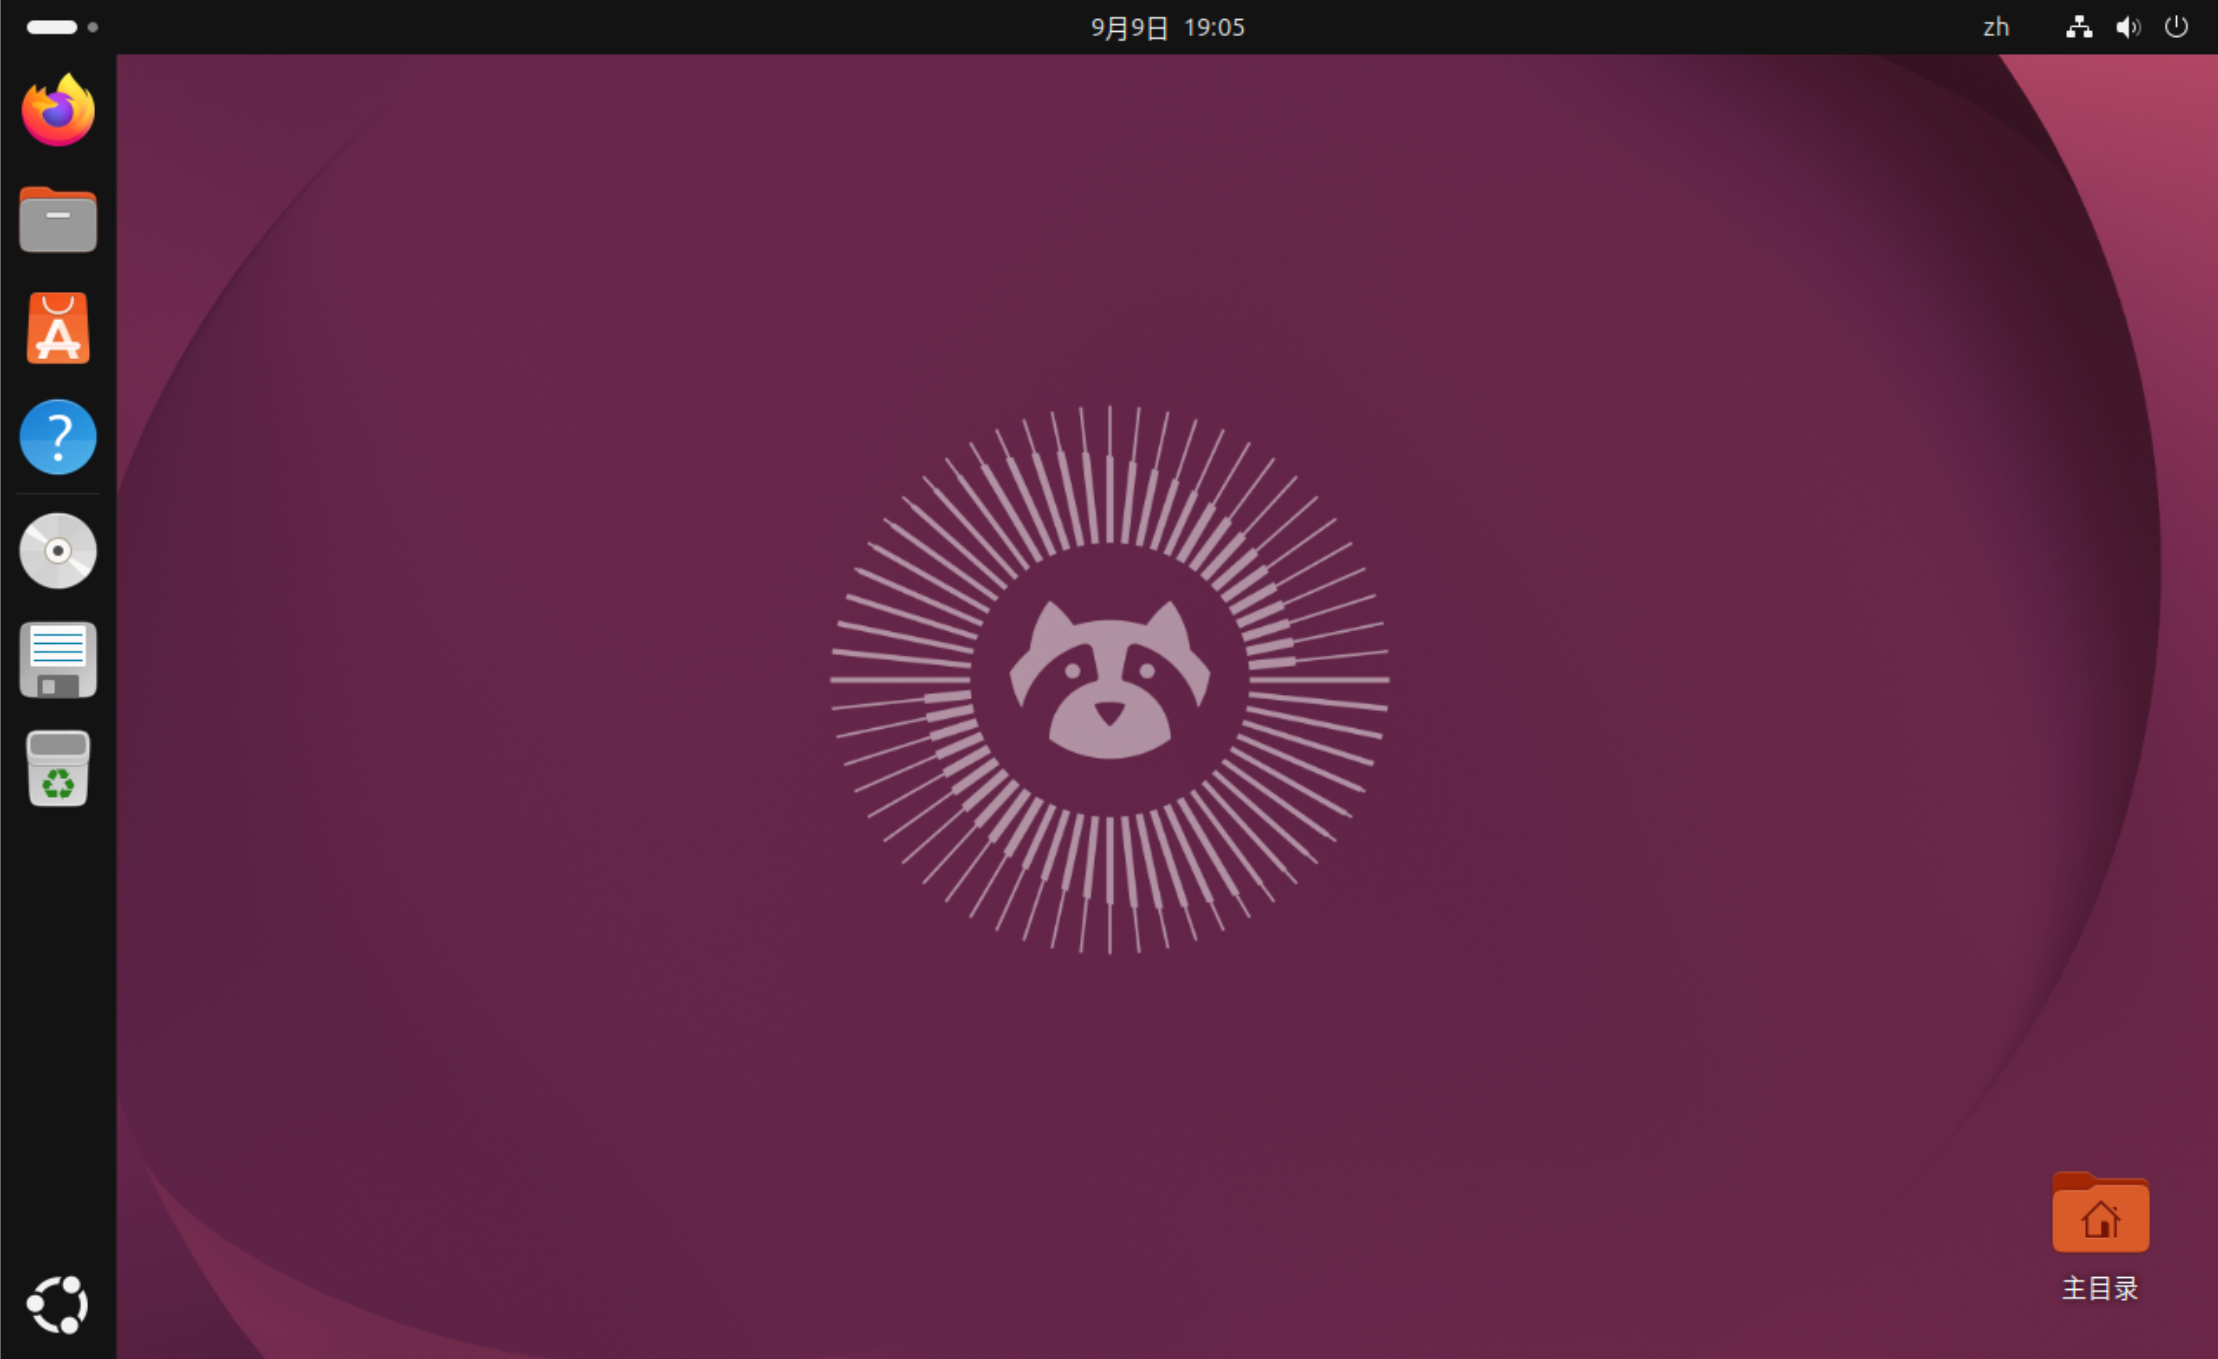
\includegraphics[width=0.8\textwidth]{Figure/Unbuntu界面.png}
  \caption{Ubuntu 桌面界面}
  \label{fig:ubuntu-desktop}
\end{figure}

\section{在 Windows 上使用 Ubuntu：WSL}

本书的最终目标，是让 ROS 2 在一套 Ubuntu 环境里跑起来。多数读者日常使用的电脑装的是 Windows，直接改装系统代价太大，装双系统又要重启切换，也谈不上方便。更轻的起步方式是：用 Windows 自带的 \textbf{WSL}，让 Ubuntu 直接住在 Windows 里。

WSL 全称 Windows Subsystem for Linux，中文叫 ``适用于 Linux 的 Windows 子系统''。一句话解释：让 Linux 直接住在 Windows 里，不必再装一台虚拟机。它开机一两秒就能进系统，能直接读写 Windows 里的文件，图形程序也能开在 Windows 桌面上。

不过这条路上的坑明显更密，几乎每走一步都会撞上一个报错。所以本章后面的环境部分不按教科书的顺序写，而是按照笔者当时真实的踩坑顺序写：先被什么卡住，屏幕上报了什么样的一段话，最后又是怎么过的。你可以把它当成一份通关记录，遇到同样的报错时直接翻到对应的小节抄命令。

\subsection{WSL 是什么}

严格说来，WSL 1 只是把 Linux 的系统调用``翻译''成 Windows 能听懂的形式，兼容性一般。从 WSL 2 开始，微软干脆在 Windows 内部塞了一台轻量虚拟机，里面跑的是真正的 Linux 内核。所以今天用的 WSL 2 和 WSL 3，本质上是``一台你看不见、也不用管的虚拟机''。

这句话很重要，因为它提前解释了后面一堆坑的共同来源：你其实是在两套系统之间来回横跳，而两边的命令、路径、权限规则全都不一样。

\begin{figure}[htbp]
\centering
\begin{tikzpicture}[font=\small,
  layer/.style={draw=black!65, rounded corners=2.5pt, minimum width=9.2cm,
                minimum height=1.0cm, align=center, text width=8.6cm, inner sep=3pt}]

\node[layer, fill=blue!10]  (win)  {Windows 11 / 10 宿主系统};
\node[layer, fill=cyan!10,  below=5mm of win]  (eng)  {WSL 引擎\\[-1pt]{\footnotesize \texttt{wsl.exe} · \texttt{WslService}}};
\node[layer, fill=teal!12,  below=5mm of eng]  (kern) {跑在轻量虚拟机里的 Linux 内核\\[-1pt]{\footnotesize 笔者的机器上为 6.18.54.1-1}};
\node[layer, fill=orange!15,below=5mm of kern] (user) {Ubuntu 26.04 用户空间\\[-1pt]{\footnotesize bash · apt · ROS 2 Lyrical}};
\node[layer, fill=green!12, below=5mm of user] (wslg) {WSLg\\[-1pt]{\footnotesize Wayland 合成器，把窗口直接摆到 Windows 桌面上}};
\end{tikzpicture}
\caption{WSL 的分层结构。Windows 里先有一层 WSL 引擎，引擎之下的 Linux 内核跑在轻量虚拟机中，内核之上才是发行版和你的程序；WSLg 负责把图形窗口送回 Windows 桌面}
\label{fig:WSL分层结构}
\end{figure}

从图~\ref{fig:WSL分层结构} 自上往下看，我们的操作其实分属不同楼层。最塌实的做法，是先记住哪条命令该在哪一层敲：

\begin{center}
\small
\begin{tabular}{|l|l|}
\hline
\textbf{在 Windows 的 PowerShell 里敲} & \textbf{在 WSL 的 Ubuntu 里敲} \\
\hline
\texttt{wsl -l -v} & \texttt{sudo apt update} \\
\texttt{wsl --update --web-download} & \texttt{systemctl --user ...} \\
\texttt{wsl --install --from-file x.wsl} & \texttt{ros2 run turtlesim ...} \\
\texttt{wsl --manage Ubuntu --move D:\textbackslash WSL} & \texttt{glxinfo -B} \\
\texttt{wsl --shutdown} & \texttt{wsl.exe --shutdown}（唯一的特例） \\
\hline
\end{tabular}
\end{center}

本章后面反复出现的报错，绝大多数都只是``在错误的楼层敲了正确的命令''而已。

\subsection{和装一台真机 Ubuntu 相比}

WSL 并不是唯一的选择，把 Ubuntu 直接装到硬盘上（单系统或双系统）也是一条路。两者差别如下：

\begin{center}
\small
\begin{tabular}{|l|l|l|}
\hline
\textbf{对比项} & \textbf{真机安装 Ubuntu} & \textbf{WSL} \\
\hline
本质 & 一台完整的电脑 & Windows 里的轻量 Linux 子系统 \\
磁盘占用 & 几十 GB 起 & 几个 GB 起 \\
开机速度 & 重启并切换系统 & 一两秒 \\
和 Windows 传文件 & 靠分区挂载或网络共享 & 直接访问 \texttt{/mnt/c} \\
图形界面 & 完整桌面，装完就有 & 单个程序开箱即用，完整桌面要折腾 \\
快照回滚 & 可用备份工具整机还原 & 没有，弄坏了只能重装 \\
\hline
\end{tabular}
\end{center}

笔者的判断是：只想跟着教程跑通 ROS 2、写几个节点，WSL 完全够用，而且比装双系统顺手得多；如果想要一台``随便怎么折腾都能救回来''的机器，那就得自己养成导出备份的习惯（本章后面会讲 \texttt{wsl --export}），或者干脆用一台独立的机器。

\section{安装并配置 WSL}

\subsection{先看清楚自己装的是哪一版}

一切从两条命令开始。第一条看引擎版本，第二条看装了哪些发行版：

\begin{lstlisting}[language=bash,title={查看 WSL 版本与已安装的发行版（在 PowerShell 中执行）}]
wsl -v
wsl -l -v
\end{lstlisting}

第一条命令会打印一大串版本号，刚看的时候一头雾水。按字段拆开就好理解了：

\begin{center}
\small
\begin{tabular}{|l|l|}
\hline
\textbf{字段} & \textbf{含义} \\
\hline
WSL 版本 & 引擎本身的版本，升级它用 \texttt{wsl --update} \\
内核版本 & 那台轻量虚拟机里跑的 Linux 内核版本 \\
WSLg 版本 & 图形界面组件的版本 \\
MSRDC / Direct3D / DXCore & 图形转发相关的组件 \\
Windows 版本 & 宿主系统版本 \\
\hline
\end{tabular}
\end{center}

第二条命令的输出，常常是新手遇到的第一个``惊吓''：

\begin{lstlisting}[language=bash,title={什么都没装时的提示}]
适用于 Linux 的 Windows 子系统没有已安装的分发。
可按照以下说明安装分发来解决此问题:
使用 'wsl.exe --list --online' 列出可用的分发
和 'wsl.exe --install <Distro>' 进行安装。
\end{lstlisting}

这其实不是报错。前面说过，WSL 引擎只是一个``壳''，Ubuntu、Debian 这些发行版是要另外装的``整车''。引擎升级和装发行版是两件独立的事，先装引擎、后装发行版完全正常。

笔者的经历就是一次典型的时间差：早上敲 \texttt{wsl -v}，显示的是 \texttt{2.7.8.0}，内核 \texttt{6.18.33.1-1}；晚上再敲，已经变成 \texttt{3.0.3.0}、内核 \texttt{6.18.54.1-1} 了。中间什么都没干，只是 Windows 自动更新顺手把 WSL 推上去了。

\subsection{从 2.7 跳到 3.0：这次升级改了什么}

从 2.7.8 一步跨到 3.0.3，看着像一次大改，其实不然。WSL 3 并不是 WSL 1 到 WSL 2 那种底层架构革命，它更像是把原本处于预览状态的容器功能正式转正，顺便把大版本号也抬了一级。

几个值得一提的变化：

\begin{itemize}
    \item \textbf{原生 Linux 容器}。新增 \verb|wslc| 命令行工具（WSL Containers），可以不装 Docker Desktop 就在 Windows 上创建、运行 Linux 容器，一行命令就能起一个 Nginx。容器也不再依赖某个特定的发行版，可以独立运行。
    \item \textbf{文件访问变快}。默认启用 virtiofs 文件系统，取代了沿用多年的 Plan 9 协议，访问 Windows 侧文件的性能官方声称最高可以翻一倍。
    \item \textbf{新的网络模式}。引入了 consomme 模式，Linux 的流量经由 Windows 主机转发，对代理服务器和企业网络策略的兼容性更好。
    \item \textbf{内核换代}。3.0 基于 Linux 6.18，并增加了自动虚拟 NUMA 支持，能在几百个线程的大型多路服务器上稳定跑。
    \item \textbf{实验性稀疏 VHD}。从 3.0.2 开始可以开启稀疏虚拟硬盘，磁盘空间按实际写入量占用，能省不少地方。
\end{itemize}

笔者用的 3.0.3 还是一个预发布（Pre-release）版本，在容器功能转正的基础上，又带了内核升级到 6.18.54.1、修复 \verb|LifetimeManager| 竞态条件、改进 \verb|wslc| 事件过滤器等一批稳定性修补。

升级命令只有一句，建议加上 \verb|--web-download|，因为默认的走法在某些网络环境下会卡住不动：

\begin{lstlisting}[language=bash,title={升级 WSL（在 PowerShell 中执行）}]
wsl --update --web-download
\end{lstlisting}

\subsection{连接要等好久，是哪里慢}

装完之后的第一感受往往不是``真快''，而是``怎么这么卡''。笔者当时的原话就是三个字：为啥连接要好久。

这件事不能笼统地问，得先判断慢在哪一环。两类情况，病因完全不同：

\begin{itemize}
    \item \textbf{启动就慢}：敲完 \verb|wsl| 回车，光标要干等十几秒才出现 Linux 提示符。这属于启动初始化问题。
    \item \textbf{启动不慢，联网慢}：很快就进系统了，但是 \verb|ping|、\verb|curl|、\verb|apt update| 一动就卡很久。这基本是网络或者 DNS 的问题。
\end{itemize}

\subsubsection{启动初始化慢}

两个容易被忽略的原因：

\begin{itemize}
    \item \textbf{断掉却还挂着的网络驱动器}。如果曾经映射过公司的 SMB 共享盘，而现在并不在同一个网络里，Windows 和 WSL 在启动时会反复尝试连接它，卡顿非常明显。把用不到的网络驱动器映射断开即可。
    \item \textbf{代理软件或 VPN 的虚拟网卡}。某些代理工具的虚拟网卡会和 WSL 的虚拟网络抢占资源，拖慢初始化。可以先把代理关掉试一次，快慢对比一下就清楚了。
\end{itemize}

\subsubsection{联网慢：网络模式与 DNS}

WSL 支持几种网络模式，默认的 NAT 模式在国内网络下经常出问题。改写配置文件 \texttt{C:\textbackslash Users\textbackslash <你的用户名>\textbackslash .wslconfig}：

\begin{lstlisting}[language=bash,title={切换为 mirrored 网络模式}]
[wsl2]
networkingMode=mirrored
\end{lstlisting}

mirrored 模式让 WSL 直接``镜像''宿主机的网络接口，能更好地兼容主机上的代理，很多莫名其妙的连接问题会随之消失。如果某个端口在 mirrored 下还是断断续续，可以再试试前面提到的 consomme 模式。

DNS 是另一个高频嫌疑。每个网络请求之前都要先解析域名，解析一慢，整体感觉就是``网卡了''。有两种处理方式：

\begin{itemize}
    \item \textbf{简单做法}：把 Windows 主机的 DNS 换成公共 DNS（比如 8.8.8.8、1.1.1.1），WSL 通常会自动继承。
    \item \textbf{彻底做法}：在 WSL 内部关掉自动生成，手动指定。编辑 \verb|/etc/wsl.conf| 加入 \verb|generateResolvConf = false|，再往 \verb|/etc/resolv.conf| 里写一行 \verb|nameserver 8.8.8.8|。
\end{itemize}

还有一种比较冷门的原因：WSL 虚拟网卡的``大量发送卸载''（LSO）在个别网络环境下反而拖后腿。用管理员权限的 PowerShell 关掉它：

\begin{lstlisting}[language=bash,title={禁用 WSL 虚拟网卡的 LSO}]
Disable-NetAdapterLso -Name "vEthernet (WSL)" -IncludeHidden
\end{lstlisting}

如果同时还在用 Docker Desktop，那 WSL 卡顿就更常见了，两者网络栈容易打架。可以到``任务管理器 \textrightarrow{} 服务''里找到 \verb|WslService| 右键重启，往往立刻见效。

最后一条与网络无关，但几乎是所有人都会犯的：\textbf{项目文件别放在 \texttt{/mnt/c} 下面}。那是 Windows 的文件系统，在它上面跑 \verb|npm install|、编译、批量读写都会慢得离谱。把项目放在 WSL 自己的家目录（比如 \verb|~/projects|），再用 VS Code 的 WSL 扩展打开，速度完全是两个世界。

\begin{center}
\small
\begin{tabular}{|l|l|}
\hline
\textbf{改了哪个文件} & \textbf{生效方式} \\
\hline
\texttt{.wslconfig} & 在 PowerShell 里执行 \texttt{wsl --shutdown} \\
\texttt{/etc/wsl.conf} & 同上 \\
\texttt{/etc/resolv.conf}（手动维护的那种） & 同上 \\
\hline
\end{tabular}
\end{center}

\subsection{安装 Ubuntu：桌面版 ISO 根本用不上}

发行版列表拉不下来，是这条路上第一个真正的拦路虎：

\begin{lstlisting}[language=bash,title={拉取发行版列表失败}]
wsl --list --online
未能从"https://raw.githubusercontent.com/microsoft/WSL/master/distributions/DistributionInfo.json"
提取分发列表。错误的网关(502)。
错误代码： Wsl/HTTP_E_STATUS_BAD_GATEWAY
\end{lstlisting}

这个 502 跟 WSL 本身没什么关系。它只是说明：你的电脑去 GitHub 取那份发行版清单时，被中间的网关拦了回来。所以从易到难依次试：

\begin{enumerate}
    \item 换用 \verb|wsl --update --web-download| 升级一次，有时候顺带就好了；
    \item 关掉代理或 VPN 再试，很多时候罪魁祸首正是它；
    \item 换 DNS，或者干脆往 \verb|hosts| 文件里手写 \verb|raw.githubusercontent.com| 的 IP；
    \item 从微软商店直接搜 Ubuntu 安装，这条路完全绕开 GitHub，最稳；
    \item 离线安装，也就是下一小节要讲的办法。
\end{enumerate}

\subsubsection{为什么 ISO 不能直接用}

笔者的第一反应很自然：我手里不是有 \verb|ubuntu-26.04.1-desktop-amd64.iso| 吗，直接装不就完了。结果是不行，而且不行得有道理。

桌面版 ISO 是一张``安装光盘''。它的内容是启动环境加一个图形化安装程序，运行起来之后要一步一步问你装到哪块硬盘、要不要格式化。而 WSL 要的东西完全不同：它需要的是一套已经装好、解压即可运行的根文件系统，直接挂起来就开机，中间没有``安装''这个步骤。

所以命令也不一样。WSL 用的是 \verb|--from-file| 或者 \verb|--import|，喂给它的必须是 \verb|.wsl| 镜像或者 rootfs 的 tar 包，不是 ISO。

\subsubsection{正确的离线安装方式}

Ubuntu 官方为每个 LTS 版本都准备了专门给 WSL 打包的镜像，文件名形如 \verb|ubuntu-26.04.1-wsl-amd64.wsl|，几百 MB，在 \verb|releases.ubuntu.com| 或者国内镜像站都能找到。下载好之后：

\begin{lstlisting}[language=bash,title={从 .wsl 镜像离线安装（在 PowerShell 中执行）}]
wsl --install --from-file "C:\Users\john\Downloads\ubuntu-26.04.1-wsl-amd64.wsl"
\end{lstlisting}

安装过程要解包并注册文件系统，会等上一两分钟。完成后会提示你创建一个 UNIX 用户名和密码，跟着走就行。

如果版本不够新、不认 \verb|--from-file| 这个参数，可以改用等价的导入方式（\verb|.wsl| 本质上就是一个 tar 归档）：

\begin{lstlisting}[language=bash,title={备选方案：手动导入}]
mkdir C:\Users\john\WSL\Ubuntu-26.04
wsl --import Ubuntu-26.04 C:\Users\john\WSL\Ubuntu-26.04 "C:\Users\john\Downloads\ubuntu-26.04.1-wsl-amd64.wsl" --version 2
\end{lstlisting}

两者有个重要区别：\textbf{用 \texttt{--import} 装出来的系统默认以 root 登录}，进去之后还得自己建一个普通用户。用 \verb|--from-file| 则会在首次启动时引导你创建用户，省事得多。

装完验证一下，看到版本号为 2 就对了：

\begin{lstlisting}[language=bash,title={验证安装结果}]
wsl -l -v
\end{lstlisting}

\subsection{把 WSL 挪到 D 盘}

WSL 的磁盘文件（\verb|ext4.vhdx|）默认塞在 C 盘的用户目录深处，用着用着 C 盘就见红了，所以迟早要挪走。先看两种办法。

\subsubsection{方法一：直接移动（首选）}

新版本的 WSL 提供了官方移动命令，一步到位，不产生中间备份文件：

\begin{lstlisting}[language=bash,title={用 --move 迁移发行版（在 PowerShell 中执行）}]
wsl --shutdown
wsl --manage Ubuntu-26.04 --move D:\WSL\Ubuntu-26.04
\end{lstlisting}

迁移完可以确认一下注册表里记的路径是不是已经改过去了：

\begin{lstlisting}[language=bash,title={查看发行版的实际存放位置}]
(Get-ChildItem HKCU:\Software\Microsoft\Windows\CurrentVersion\Lxss |
  Where-Object { $_.GetValue("DistributionName") -eq 'Ubuntu-26.04' }).GetValue("BasePath")
\end{lstlisting}

返回 \verb|D:\WSL\Ubuntu-26.04| 就说明成功了。如果报 \verb|ERROR_FILE_NOT_FOUND| 之类的错误，说明注册表没更新干净，那就改用方法二。

\subsubsection{方法二：导出再导入（最稳）}

这个办法的原理是``先打包备份，再解包到新位置''，兼容性最好，也最让人放心：

\begin{lstlisting}[language=bash,title={导出、注销、再导入}]
mkdir D:\WSL_Backup
wsl --export Ubuntu-26.04 D:\WSL_Backup\ubuntu-backup.tar
wsl --unregister Ubuntu-26.04
mkdir D:\WSL\Ubuntu-26.04
wsl --import Ubuntu-26.04 D:\WSL\Ubuntu-26.04 D:\WSL_Backup\ubuntu-backup.tar
\end{lstlisting}

注意中间那一步 \verb|--unregister| 会真的把 C 盘上的原系统删掉，执行之前一定确认备份文件已经生成好了。导入之后同样会变成 root 登录，需要重新配置默认用户。

如果还没装、想一步到位装在 D 盘，安装时直接带上 \verb|--location| 参数即可：

\begin{lstlisting}[language=bash,title={全新安装并指定位置}]
wsl --install -d Ubuntu-26.04 --location D:\WSL\Ubuntu-26.04
\end{lstlisting}

\subsubsection{一个特别典型的误会}

笔者当时在 WSL 里敲了这么一行，然后被权限拒绝：

\begin{lstlisting}[language=bash,title={错误示范}]
mkdir /opt/WSL
mkdir: Permission denied
\end{lstlisting}

表面上是权限问题（\verb|/opt| 是系统目录，普通用户写不进去，需要 \verb|sudo|），但真正的问题是层次搞错了：\verb|/opt/WSL| 是 \textbf{Linux 文件系统里}的一个目录，它实际存在 C 盘那个 \verb|ext4.vhdx| 里面，跟 Windows 的 D 盘一点关系都没有。想迁移到 D 盘，必须回到 PowerShell 那边去操作。

判断自己要做哪件事，看这张表就够了：

\begin{center}
\small
\begin{tabular}{|l|l|l|}
\hline
\textbf{你想做的事} & \textbf{在哪敲} & \textbf{命令} \\
\hline
在 Linux 里建个文件夹 & WSL 的 bash & \texttt{sudo mkdir /opt/WSL} \\
把整个发行版迁到 D 盘 & Windows PowerShell & \texttt{wsl --manage ... --move ...} \\
访问 D 盘上的文件 & WSL 的 bash & 直接进 \texttt{/mnt/d/...} \\
\hline
\end{tabular}
\end{center}

\section{中文显示和中文输入}

系统装好、能进 bash 了，下一步自然是让它能好好显示中文。这件事其实分三层，很多人把三层混在一起，于是装了一堆互相打架的包。

\begin{enumerate}
    \item \textbf{locale}：决定系统用什么语言、什么编码，关系到日期格式、排序、提示信息；
    \item \textbf{字体}：决定汉字有没有字形可以画出来，缺字体就显示成方块；
    \item \textbf{输入法}：决定你怎么把中文敲进去。
\end{enumerate}

\subsection{第一课：apt 必须 sudo}

拦在第一道的是权限，而且报错信息长得很唬人：

\begin{lstlisting}[language=bash,title={apt 的权限报错}]
Error: Could not open lock file /var/lib/dpkg/lock-frontend - open (13: Permission denied)
Error: Unable to acquire the dpkg frontend lock (/var/lib/dpkg/lock-frontend), are you root?
\end{lstlisting}

意思很直白：装软件要动 \verb|/var/lib/dpkg| 这类系统目录，普通用户没有权限，拿不到那把``锁''。命令前面加 \verb|sudo| 就好。

\subsection{第二课：包名对不上，整条命令全废}

这条坑很值得单独说。笔者当时一口气装了一串包：

\begin{lstlisting}[language=bash,title={看起来没问题的命令}]
sudo apt install xfonts-wqy xfonts-unifont fonts-wqy
\end{lstlisting}

结果只有一句 \verb|Unable to locate package fonts-wqy|。看起来只是少装一个包，其实不是：\textbf{apt 只要在一条命令里遇到一个找不到的包，整条命令就会整体失败}。也就是说 \verb|xfonts-wqy| 和 \verb|xfonts-unifont| 一个都没装上。

原因是 Ubuntu 里压根没有叫 \verb|fonts-wqy| 的包，文泉驿字体是拆开成好几个子包的。正确的写法是：

\begin{lstlisting}[language=bash,title={分两条，先装 X 字体，再装真正有用的字体}]
sudo apt install xfonts-wqy xfonts-unifont
sudo apt install fonts-wqy-zenhei fonts-wqy-microhei fonts-noto-cjk
\end{lstlisting}

顺带解释一下这两类的区别：\verb|xfonts-*| 是旧式的 X 核心字体，对 gedit 这类现代 GTK 程序帮助很有限；真正起作用的是 fontconfig 体系下的字体，其中 \verb|fonts-noto-cjk| 是显示中文的主力，比文泉驿完整得多。

\subsection{第三课：语言包和 locale}

语言包提供的是``语言数据''，管的是菜单、对话框有没有中文翻译：

\begin{lstlisting}[language=bash,title={安装中文语言包并设定默认 locale}]
sudo apt update
sudo apt install language-pack-gnome-zh-hans language-pack-zh-hans
sudo update-locale LANG=zh_CN.UTF-8
\end{lstlisting}

有两点要留意。一是 \verb|language-pack-kde-zh-hans| 在 Ubuntu 官方源里通常找不到，它属于 Kubuntu 的源，直接装会报错，用 GNOME 的话压根不需要。二是 \verb|update-locale| 写进的是下次登录才读的配置，当前这个终端不会立刻变，退出重进或者 \verb|wsl --shutdown| 之后才生效，用 \verb|locale| 命令可以确认。

\subsection{第四课：输入法，别装}

这是笔者绕得最远的一个弯。当时想当然地装了一整套 fcitx：\verb|fcitx|、\verb|fcitx-config-gtk|、\verb|fcitx-sunpinyin|、\verb|fcitx-googlepinyin|，结果发现是个反方向的努力。

因为 \textbf{WSLg 已经把 Windows 的输入法桥接进来了}。在 WSL 里运行的 Linux 图形程序，直接按 Windows 自己的输入法切换键就能打中文，根本不需要在 Linux 内部再养一套输入法。反过来，装了 fcitx 还会跟 WSLg 的桥接机制抢键盘，弄不好两边都失效。

所以结论就一句：\emph{输入法一个都不要装}。要装的只有字体和语言包。

\section{wsl --shutdown 到底敲在哪}

改完 locale，按照惯例要重启 WSL 让配置生效。于是笔者在 Ubuntu 的 bash 里敲了：

\begin{lstlisting}[language=bash,title={一个必然失败的尝试}]
wsl --shutdown
Command 'wsl' not found, but can be installed with:
sudo apt install wsl
\end{lstlisting}

两个要点。

第一，\verb|wsl| 是 Windows 侧的命令，你现在在 Linux 里，当然找不到。正确做法是在 PowerShell 或 CMD 里敲。

第二，那句``可以 sudo apt install wsl''是个陷阱，\textbf{千万别照做}。Ubuntu 软件源里确实有个叫 \verb|wsl| 的包，但它跟微软的 WSL 毫无关系，装上去什么用都没有，只会让以后查问题时多一层混淆。

如果实在不想切窗口，还有个取巧的办法：WSL 支持直接调用 Windows 的可执行文件（这叫 interop），所以带上 \verb|.exe| 后缀就能在 bash 里执行：

\begin{lstlisting}[language=bash,title={在 Linux 里调用 Windows 命令}]
wsl.exe --shutdown
\end{lstlisting}

只是这么一来，当前会话会被自己关掉，终端直接退出。另外，如果目的只是让新配置生效，其实用不着 shutdown，把终端窗口关掉再开一个就够了。

\section{gedit 后面那串奇怪字符}

启动 gedit 之后，终端里喷出来一堆这样的东西：

\begin{lstlisting}[language=bash,title={终端里刷出来的一串控制序列}]
gedit;28;13;1;32;1_;28;13;0;32;1_;14;8;1;32;1_;14;8;0;32;1_;
\end{lstlisting}

看着像乱码，其实不是。这些是应用程序发给终端的 \textbf{ANSI 控制序列}，本意是控制光标位置、颜色、清屏之类的动作，正常情况下应该被终端``解析并执行''，而不是打印出来。之所以原形毕露，是因为 gedit 察觉到自己接的不是一个真正的交互式终端，于是干脆把原始指令直接输出了。

它既不影响使用，也不说明程序坏了。嫌吵的话，把输出丢掉或者让它脱离当前会话就行：

\begin{lstlisting}[language=bash,title={两种清静的办法}]
gedit 2>/dev/null
setsid gedit
\end{lstlisting}

真正需要警惕的是另一种情况：如果 gedit 窗口里的汉字变成了方块，那才是字体没装好，回去补 \verb|fonts-noto-cjk|。

\section{在 WSLg 里跑出一整个 GNOME 桌面}

到这里为止，WSL 已经能跑单个图形程序了。但笔者贪心，想要一整个 Ubuntu 桌面，跟真机装完系统那样。这件事能做成，但要做好折腾一下午的心理准备。

先说一个必须绕开的坑：从网上找到项目地址，直接把 URL 粘到终端里回车。

\begin{lstlisting}[language=bash,title={把网址当命令敲}]
https://github.com/nufeng1999/WSL_GNOME
-bash: https://github.com/nufeng1999/WSL_GNOME: 没有那个文件或目录
\end{lstlisting}

Shell 不认识 \verb|https://| 开头的东西，网址不是可执行程序。要用它，得先 \verb|git clone| 下来，再执行里面的脚本。

\subsection{两条路，选哪条}

\begin{center}
\small
\begin{tabular}{|l|l|l|}
\hline
\textbf{方案} & \textbf{原理} & \textbf{维护状态} \\
\hline
WSL\_GNOME & 借助 Cygwin 的 XWin 提供 X 服务 & 2021 年后基本停更 \\
WSLg 原生 & WSLg 的 Wayland 合成器直接跑 GNOME & 社区活跃 \\
\hline
\end{tabular}
\end{center}

笔者的 WSL 已经是 3.0.3，自带 WSLg，所以最后走的是右边这条。下面记的就是这条路的完整过程，也算给 Ubuntu 26.04 这个比较新的组合留一份记录。

\subsection{准备工作}

首先要打开 systemd。GNOME 的会话是 systemd 用户服务，没有 systemd 就无从谈起。编辑 \verb|/etc/wsl.conf|：

\begin{lstlisting}[language=bash,title={启用 systemd}]
[boot]
systemd=true
\end{lstlisting}

改完在 PowerShell 里 \verb|wsl --shutdown|，重新进来才会生效。

然后装桌面。这里有个关键包 \verb|mutter-dev-bin|，不能漏：

\begin{lstlisting}[language=bash,title={安装桌面环境}]
sudo apt update
sudo apt install ubuntu-desktop mutter-dev-bin
\end{lstlisting}

\verb|mutter-dev-bin| 之所以关键，是因为 Ubuntu 26.04 带的是 GNOME 50，而 GNOME 从 49 之后彻底移除了旧的 \verb|--nested| 参数，改用 \verb|--devkit| 模式来启动嵌套桌面，这个参数正是由 \verb|mutter-dev-bin| 提供的。少装它，后面的启动命令一定失败。

还有一步容易被忽略：把 GDM 屏蔽掉。GDM 是 Ubuntu 的登录管理器，在 WSLg 下面无法正常工作，反而会挡住后面手动启动的会话。

\begin{lstlisting}[language=bash,title={屏蔽 GDM 并降低渲染要求}]
sudo systemctl mask gdm.service
echo 'export GSK_RENDERER=cairo' >> ~/.bashrc
source ~/.bashrc
\end{lstlisting}

\verb|GSK_RENDERER=cairo| 是给 GTK4 应用用的保险，能避开 WSL 下 GPU 渲染导致的卡死和黑屏。

\subsection{让 GNOME Shell 用正确的方式启动}

接下来要覆盖 \verb|gnome-shell| 的启动命令，强制它走 \verb|--devkit --no-x11| 这条路：

\begin{lstlisting}[language=bash,title={创建 systemd 覆盖文件}]
sudo mkdir -p /etc/systemd/user/org.gnome.Shell@.service.d/
sudo nano /etc/systemd/user/org.gnome.Shell@.service.d/override.conf
\end{lstlisting}

文件内容是这样，注意第一行 \verb|ExecStart=| 后面是空的：

\begin{lstlisting}[language=bash,title={override.conf}]
[Service]
ExecStart=
ExecStart=/usr/bin/gnome-shell --devkit --no-x11 --mode=%i
\end{lstlisting}

那行空的 \verb|ExecStart=| 不是笔误，也绝对不能省。systemd 的规则是：同名的 \verb|ExecStart| 会累加执行，只有先写一个空的把默认值清掉，后面这行才会成为唯一的启动命令。

在 nano 里保存退出的手法是：\verb|Ctrl+O| 写入、回车确认文件名，然后 \verb|Ctrl+X| 退出。

\subsection{排错一：snap 卡在 0\%，然后把 dpkg 搞坏了}

装 \verb|ubuntu-desktop| 的过程中，屏幕卡在了这么一行：

\begin{lstlisting}[language=bash,title={卡住的 snap 下载}]
==> Installing the firefox snap
下载 snap "snapd" (28254)，来自频道 "stable"
进度：[  0%] [
\end{lstlisting}

原因是 Ubuntu 26.04 里的 \verb|firefox| 已经是一个 snap 过渡包，安装时要去 snap 商店现场下载本体，而 snap 在国内没有官方镜像，速度很不稳定。卡在 0\% 通常就是它在等一个永远等不到的连接。

最要命的是后续：下载连接被重置，安装脚本失败，整个 \verb|dpkg| 的配置流程就中断了，此后所有 apt 操作都会报依赖损坏。

修复顺序是这样的：

\begin{lstlisting}[language=bash,title={修复被中断的 dpkg，并强制移除坏掉的 firefox}]
sudo dpkg --configure -a
sudo apt --fix-broken install
sudo dpkg --force depends -P firefox
\end{lstlisting}

然后绕开 firefox 重新装桌面。apt 支持在包名后面加一个减号表示``不要装这个''：

\begin{lstlisting}[language=bash,title={排除 firefox 和 thunderbird 再装桌面}]
sudo apt install ubuntu-desktop firefox- thunderbird-
\end{lstlisting}

如果确实需要一个能用的 Firefox，可以改用 Mozilla 官方 PPA 提供的传统 deb 版本，这样就完全不走 snap 了：

\begin{lstlisting}[language=bash,title={用 PPA 安装 deb 版 Firefox}]
sudo add-apt-repository ppa:mozillateam/ppa
sudo apt update
sudo apt install firefox
\end{lstlisting}

另外几条缓解 snap 卡顿的办法也记在这里：

\begin{itemize}
    \item 重启 snapd 服务：\verb|sudo systemctl restart snapd snapd.socket|；
    \item 清掉缓存的 snap 文件：\verb|sudo rm -rf /var/lib/snapd/cache/*|；
    \item 给 snapd 单独配上代理。
\end{itemize}

\subsection{排错二：asserts failed}

配置都写好了，敲下启动命令，等来的却是这样一句：

\begin{lstlisting}[language=bash,title={启动桌面失败}]
systemctl --user daemon-reload
systemctl --user start gnome-session@ubuntu.target
A dependency job for gnome-session@ubuntu.target failed. See 'journalctl -xe' for details.
\end{lstlisting}

先别猜，直接看日志：

\begin{lstlisting}[language=bash,title={查日志}]
journalctl --user -u gnome-session@ubuntu.target -u org.gnome.Shell@ubuntu.service --no-pager -n 50
\end{lstlisting}

日志里有价值的是这三行：

\begin{lstlisting}[language=bash,title={日志里的关键三行}]
org.gnome.Shell@ubuntu.service: Starting requested but asserts failed.
Assertion failed for org.gnome.Shell@ubuntu.service - GNOME Shell.
Dependency failed for gnome-session@ubuntu.target - GNOME Session (session: ubuntu).
\end{lstlisting}

\verb|asserts failed| 的意思是：服务启动前有个前置条件没满足，systemd 干脆不让它启动。GNOME Shell 的服务单元里带着一条断言，要求环境变量 \verb|XDG_SESSION_TYPE| 必须是 \verb|wayland|。而在 WSLg 环境下，这个变量没有被正确送进 systemd 的用户会话里，断言自然就挂了。

补上它就行。systemd 用户会话会在启动时读取 \verb|~/.config/environment.d/| 下面的配置，把变量写进去：

\begin{lstlisting}[language=bash,title={补上缺失的会话类型变量}]
mkdir -p ~/.config/environment.d/
nano ~/.config/environment.d/gnome-wayland.conf
\end{lstlisting}

内容：

\begin{lstlisting}[language=bash,title={gnome-wayland.conf}]
XDG_SESSION_TYPE=wayland
XDG_SESSION_DESKTOP=gnome
XDG_CURRENT_DESKTOP=GNOME
\end{lstlisting}

然后重载再启动：

\begin{lstlisting}[language=bash,title={重新拉起桌面}]
systemctl --user daemon-reload
systemctl --user start gnome-session@ubuntu.target
\end{lstlisting}

这一次桌面就真的出来了。事后回看，卡了半天的只是三个环境变量。

\subsection{桌面跑起来之后}

几条经验，都是踩出来的：

\begin{itemize}
    \item \textbf{给它起个别名}。启动命令太长，写进 \verb|~/.bashrc|：\verb|alias startgnome='systemctl --user start gnome-session@ubuntu.target'|，以后一句 \verb|startgnome| 就能呼出桌面。
    \item \textbf{千万别点``注销''或``重启系统''}。WSL 里没有登录管理器接管，桌面窗口一关就再也不会自己弹回来，还得回终端重新敲启动命令。
    \item \textbf{卡死了就 \texttt{wsl --shutdown}}。关掉等几秒再进，比在桌面里点什么都管用。
    \item \textbf{平时可以不启动桌面}。纯命令行开发完全不需要它，桌面是要吃 CPU 和内存的。
\end{itemize}

\section{ROS 是什么}

\subsection{ROS 不是操作系统}

ROS 的全称是 Robot Operating System，中文常译作``机器人操作系统''。这个叫法很有迷惑性：\emph{ROS 并不是一个操作系统}，它不能独立安装在裸机上，而是运行在操作系统（通常是 Ubuntu）之上的一套\emph{开源机器人软件开发框架}。ROS本身并不是一个操作系统，而是可以安装在现在已有的操作系统上（Linux、Windows、Mac）上的 软件库和工具集 。

为什么机器人软件需要这样一套框架？因为一个稍微像样的机器人程序，往往由很多独立的部分组成：读取激光雷达和相机数据、处理感知、做运动规划、控制电机、与人交互……如果每个模块都自己写一套和别人通信的办法，整个系统会迅速变成一团乱麻。ROS 要解决的正是这个问题：它规定了一套统一的通信机制，并提供了大量现成的工具和功能包，让开发者可以专心写自己的那一部分，其余交给生态。

\subsection{核心概念：节点与通信}

ROS 里有两个必须最先建立印象的概念：

\begin{itemize}
    \item \textbf{节点（node）}：一个可以独立运行的程序模块。整个机器人系统可以看作许多节点协作组成的 ``网络''。
    \item \textbf{通信方式}：节点之间通过\emph{话题（topic）}、\emph{服务（service）}、\emph{动作（action）}等方式交换\emph{消息（message）}，消息就是节点间传递的数据包。
\end{itemize}

打个比方：传感器节点像是不断播报路况的广播电台（话题），导航节点像是收听广播的司机；而当你需要打车时那种``一问一答''的交互（服务），又和广播完全不同。这套通信机制的细节会在后面的章节展开，这里先记住``节点 + 通信''这个总框架即可。

\subsection{从 ROS 1 到 ROS 2}

ROS 起源于 2007 年斯坦福大学的一个机器人项目，随后由 Willow Garage 公司推动，逐渐发展成全球机器人研究界的事实标准，积累了庞大的生态。不过随着机器人应用走向工业化和复杂化，ROS 1 的一些先天设计问题开始暴露：

\begin{itemize}
    \item 通信依赖一个中心节点 \texttt{roscore}，它一旦宕机，整个系统就瘫痪；
    \item 以单机为主，多机分布式和实时性支持不足；
    \item 几乎没有安全机制，难以满足工业级要求。
\end{itemize}

于是社区从 2014 年前后开始重新设计，2017 年发布了 ROS 2 的第一个正式发行版。ROS 2 不是 ROS 1 的小修小补，而是一次架构级的重写。今天，ROS 1 已经停止维护（最后一个发行版是 2020 年的 Noetic），新项目都应当基于 ROS 2。本书讲的也是 ROS 2。

\section{ROS 1 与 ROS 2 的主要区别}

把上面的要点归纳成一张对比表，方便查阅：

\begin{center}
\begin{tabular}{|l|l|l|}
\hline
\textbf{对比项} & \textbf{ROS 1} & \textbf{ROS 2} \\
\hline
通信机制 & 自研 TCPROS/UDPROS & 基于 DDS 标准 \\
中心节点 & 依赖 \texttt{roscore} & 去中心化，无需主节点 \\
实时性 & 不支持 & 可通过 DDS 配置支持 \\
多机分布式 & 支持较弱 & 原生良好支持 \\
安全机制 & 几乎没有 & 内置（如 SROS2） \\
支持平台 & 主要 Linux & Linux/Windows/macOS 等 \\
\hline
\end{tabular}
\end{center}

对学习者而言，这些区别并不需要现在就全部弄懂。你只需要记住一个大方向：\emph{学 ROS 2}。后面章节里出现的所有命令和示例，都默认运行在 ROS 2 之上。

\section{ROS 2 与 Ubuntu 版本的搭配}

ROS 2 和 Ubuntu 一样，也有发行版的概念，而且两者高度绑定：官方每两年发布一个 ROS 2 的 LTS 版本，与当年度 Ubuntu 的 LTS 版本一一对应。最常用的组合如下：

\begin{center}
\begin{tabular}{|l|l|l|}
\hline
\textbf{Ubuntu 版本} & \textbf{ROS 2 发行版} & \textbf{说明} \\
\hline
20.04（2020 LTS） & Foxy（2020 LTS） & 较旧，已停止维护 \\
22.04（2022 LTS） & Humble（2022 LTS） & 目前最主流，教程最多 \\
24.04（2024 LTS） & Jazzy（2024 LTS） & 最新，适合新硬件 \\
26.04（2026 LTS） & Lyrical（2026 LTS） & 本书使用的组合 \\
\hline
\end{tabular}
\end{center}

给初学者的建议很明确：\emph{Ubuntu 22.04 + ROS 2 Humble} 是目前资料最全、社区最活跃、兼容性问题最少的组合。如果你的电脑比较新，或者像本章一样用 WSL 装了 26.04，那就跟着 26.04 + Lyrical 走；下面给出的安装命令也都是以 Lyrical 为例。

这里有一条最重要的原则：\emph{不要混搭}。比如在 Ubuntu 20.04 上硬装 Humble，或在 22.04 上装 Foxy，往往会遇到一堆莫名其妙的编译错误，而问题根源只是版本不对。版本搭配对了，后面能少走一半弯路。等你在第二章学会打开终端之后，可以用 \texttt{lsb\_release -a} 这条命令随时查看自己系统的 Ubuntu 版本。

\section{在 WSL 里安装 ROS 2}

终于到了正题。前面说过 ROS 2 和 Ubuntu 是严格配对的，所以第一步永远是确认系统版本。

这一条千万记住：\textbf{版本对不上，装是装不上的}。在 26.04 上敲 \verb|apt install ros-humble-desktop|，得到的只会是 \verb|Unable to locate package|，因为软件源里根本没有为这个系统编译的 Humble 包。

\subsection{官方路线：ros2-apt-source}

ROS 2 官方现在的推荐做法，是用一个叫 \verb|ros2-apt-source| 的配置包自动帮你把软件源和 GPG 密钥都配好，不用再手工拼源地址：

\begin{lstlisting}[language=bash,title={自动配置 ROS2 软件源}]
sudo apt install curl -y
export ROS_APT_SOURCE_VERSION=$(curl -s https://api.github.com/repos/ros-infrastructure/ros-apt-source/releases/latest | grep -F "tag_name" | awk -F'"' '{print $4}')
curl -L -o /tmp/ros2-apt-source.deb "https://github.com/ros-infrastructure/ros-apt-source/releases/download/${ROS_APT_SOURCE_VERSION}/ros2-apt-source_${ROS_APT_SOURCE_VERSION}.$(. /etc/os-release && echo ${UBUNTU_CODENAME:-${VERSION_CODENAME}})_all.deb"
sudo dpkg -i /tmp/ros2-apt-source.deb
sudo apt update
\end{lstlisting}

这条路干净利落，但它有一个前提：连得上 GitHub。笔者这里就翻车了：

\begin{lstlisting}[language=bash,title={连不上 GitHub}]
curl: (7) Failed to connect to github.com port 443 after 3 ms: Could not connect to server
\end{lstlisting}

那就换国内的镜像源走。

\subsection{国内镜像路线}

思路很简单：自己把密钥和源地址写进去，跳过 GitHub。用清华源举例：

\begin{lstlisting}[language=bash,title={从清华镜像取密钥并转换格式}]
sudo rm -f /usr/share/keyrings/ros-archive-keyring.gpg
sudo rm -f /etc/apt/sources.list.d/ros2.list
curl -sSL https://mirrors.tuna.tsinghua.edu.cn/rosdistro/ros.key | sudo gpg --dearmor -o /usr/share/keyrings/ros-archive-keyring.gpg
echo "deb [arch=$(dpkg --print-architecture) signed-by=/usr/share/keyrings/ros-archive-keyring.gpg] https://mirrors.tuna.tsinghua.edu.cn/ros2/ubuntu $(lsb_release -cs) main" | sudo tee /etc/apt/sources.list.d/ros2.list > /dev/null
sudo apt update
\end{lstlisting}

这里藏着一个非常值得记住的坑。如果只是把 \verb|ros.key| 下载下来直接丢进 \verb|keyrings| 目录，\verb|apt update| 会给你这样一段：

\begin{lstlisting}[language=bash,title={密钥格式不对时的报错}]
Err:4 https://mirrors.tuna.tsinghua.edu.cn/ros2/ubuntu resolute InRelease
  The following signatures couldn't be verified because the public key is not available:
  NO_PUBKEY F42ED6FBAB17C654
Warning: The key(s) in the keyring /usr/share/keyrings/ros-archive-keyring.gpg
  are ignored as the file has an unsupported filetype.
Error: The repository '...' is not signed.
Error: Unable to locate package ros-lyrical-desktop
\end{lstlisting}

关键字是 \verb|unsupported filetype|。新版 apt 要求密钥文件必须是二进制格式，而官网给的 \verb|ros.key| 是 ASCII 文本。中间那一步 \verb|gpg --dearmor| 就是干这个转换的，少了它，密钥等于没装。\verb|NO_PUBKEY| 和 \verb|Unable to locate package| 都是它的连锁反应。

\subsection{安装并验证}

源通了之后，装桌面版，它包含 RViz2、rqt、demos 等全套工具：

\begin{lstlisting}[language=bash,title={安装 ROS2 Lyrical 桌面版}]
sudo apt install ros-lyrical-desktop -y
\end{lstlisting}

这个过程会顺带把 OpenJDK、点云库 PCL、可视化库 VTK 等一大堆依赖一起装上，输出能刷几百行，看到 \verb|Setting up ros-lyrical-desktop| 就说明成了。

然后配环境变量，让每个新终端都认识 \verb|ros2| 命令：

\begin{lstlisting}[language=bash,title={配置环境变量}]
echo "source /opt/ros/lyrical/setup.bash" >> ~/.bashrc
source ~/.bashrc
\end{lstlisting}

验证还是老一套的``你说我听''，开两个终端：

\begin{lstlisting}[language=bash,title={验证安装}]
# 终端 1：发布者
ros2 run demo_nodes_cpp talker

# 终端 2：订阅者
ros2 run demo_nodes_py listener
\end{lstlisting}

看到一边刷 \verb|Publishing: 'Hello World: 1'|、另一边刷 \verb|I heard: [Hello World: 1]|，就成功了。

\subsection{如果两个节点互相听不见}

这一步在 WSL 里失败的概率不低，而且现象很迷惑：两个节点都正常跑着，就是收不到消息。

原因出在 WSL 默认的 NAT 网络模式上。ROS 2 底层靠 DDS 通信，节点之间要靠多播互相发现，而 NAT 模式会把这个过程挡住。解决办法还是那条：在 \texttt{C:\textbackslash Users\textbackslash <你的用户名>\textbackslash .wslconfig} 里改成镜像模式，然后 \verb|wsl --shutdown| 重启。

\begin{lstlisting}[language=bash,title={.wslconfig}]
[wsl2]
networkingMode=mirrored
\end{lstlisting}

第四章还会介绍鱼香 ROS 的一键安装脚本，那是另一种更省事的装法，两条路殊途同归；无论走哪条，验证方式都是上面这段``你说我听''。

\section{让 rviz2 正常出图}

最后一个坑，也是笔者花了最多时间的一个。小海龟能正常跑，说明 WSLg 的图形转发没问题；但一敲 \verb|rviz2|，就是这条：

\begin{lstlisting}[language=bash,title={rviz2 启动失败}]
Invalid parentWindowHandle (wrong server or screen) in GLXWindow::create
\end{lstlisting}

这个错误的根子在 rviz2 用的 Ogre 渲染引擎和 WSLg 默认的 Wayland 协议之间。Ogre 想按老一套 X11 的方式去创建窗口，结果拿到的窗口句柄``不是它熟悉的那个''。

\subsection{第一招：强制走 XCB}

最直接的办法，是让 Qt 程序改用更成熟的 X11 后端，绕开 Wayland 那条路：

\begin{lstlisting}[language=bash,title={强制使用 XCB 后端}]
export QT_QPA_PLATFORM=xcb
rviz2
\end{lstlisting}

有效的话就写进 \verb|~/.bashrc| 长期保留。不过要提醒一句，这个变量是给 rviz2 这类基于 Qt 和 Ogre 的程序用的，\textbf{不建议}全局常开，它会影响其他本来就适配良好的 Wayland 应用。

\subsection{第二招：补图形库，并让 Mesa 用上显卡}

如果第一招没用，就检查 OpenGL 这一层。这里遇到的第一个报错是包名过期：

\begin{lstlisting}[language=bash,title={libgl1-mesa-glx 已经不存在了}]
Error: Package 'libgl1-mesa-glx' has no installation candidate
\end{lstlisting}

\verb|libgl1-mesa-glx| 这个包从 Ubuntu 23.10 起就被废弃了，现在的对应物是 \verb|libgl1| 和 \verb|libglx-mesa0|：

\begin{lstlisting}[language=bash,title={正确的包名}]
sudo apt update
sudo apt install libgl1 libglx-mesa0 libgl1-mesa-dri mesa-utils
\end{lstlisting}

装完还要多做一步。WSLg 里 Mesa 默认不一定挑中 D3D12 这条通显卡的路，可能悄悄退回 \verb|llvmpipe|，也就是纯 CPU 软件渲染。软件渲染也能画，但帧率会难看得让人怀疑人生，所以显式指定驱动：

\begin{lstlisting}[language=bash,title={让 Mesa 走 D3D12}]
echo 'export GALLIUM_DRIVER=d3d12' >> ~/.bashrc
source ~/.bashrc
\end{lstlisting}

验证方式是把当前渲染器打出来：

\begin{lstlisting}[language=bash,title={查看当前使用的 OpenGL 渲染器}]
glxinfo -B | grep -E "OpenGL renderer|Device"
\end{lstlisting}

笔者的机器上输出是：

\begin{lstlisting}[language=bash,title={硬件加速已生效}]
    Device: D3D12 (NVIDIA GeForce RTX 4060 Laptop GPU) (0xffffffff)
OpenGL renderer string: D3D12 (NVIDIA GeForce RTX 4060 Laptop GPU)
\end{lstlisting}

看到 \verb|D3D12| 加上自己的显卡型号，就说明 GPU 直通已经工作了。如果这里显示的是 \verb|llvmpipe|，那说明还在软件渲染，回头检查 \verb|GALLIUM_DRIVER| 有没有生效。

\subsection{最后一招：软件渲染兜底}

如果显卡这条路怎么都不通，那还有最后的退路，牺牲性能换能用：

\begin{lstlisting}[language=bash,title={强制软件渲染}]
LIBGL_ALWAYS_SOFTWARE=1 rviz2
\end{lstlisting}

这只适合应急，界面的卡顿会非常明显，别当长期方案。

\section{这一路的坑，一张表收尾}

把上面所有的报错和原因压缩成一张速查表，下次遇到直接查：

\begin{center}
\small
\begin{tabular}{|p{4.2cm}|p{4.4cm}|p{5.6cm}|}
\hline
\textbf{现象} & \textbf{真正原因} & \textbf{一句话解决} \\
\hline
\texttt{wsl --list --online} 报 502 & 连不上 GitHub & 关代理，或直接离线装 \\
桌面版 ISO 装不进 WSL & ISO 是安装程序，不是根文件系统 & 下 \texttt{.wsl} 镜像，用 \texttt{--from-file} \\
\texttt{mkdir /opt} 权限拒绝 & 没 sudo；且路径与 D 盘无关 & 加 sudo，迁移回 PowerShell 做 \\
apt 报 \texttt{dpkg lock} 权限错 & 没加 sudo & 命令前加 sudo \\
一条 apt 命令什么都没装上 & 其中有个包名不存在，整条失败 & 拆开逐条装，先确认包名 \\
中文显示成方块 & 缺字体 & 装 \texttt{fonts-noto-cjk} \\
装了 fcitx 打不出中文 & 与 WSLg 的输入法桥接冲突 & 卸掉，直接用 Windows 输入法 \\
\texttt{wsl --shutdown} 找不到命令 & 在 Linux 侧敲了 Windows 命令 & 去 PowerShell，或敲 \texttt{wsl.exe} \\
\texttt{gedit} 后面一串分号数字 & ANSI 控制序列被原样打印 & 无需处理，或 \texttt{2>/dev/null} \\
终端里敲网址报``没有那个文件或目录'' & 把网址当命令了 & 先 \texttt{git clone} \\
snap 卡在 0\% & 国内访问 snap 商店不稳定 & 重启 snapd，或用 PPA 装 deb 版 \\
桌面起不来，日志写 asserts failed & 缺 \texttt{XDG\_SESSION\_TYPE} & 写进 \texttt{environment.d} \\
\texttt{NO\_PUBKEY} / unsupported filetype & 密钥是文本格式 & \texttt{gpg --dearmor} 转二进制 \\
两个节点互相听不见 & NAT 挡了 DDS 多播 & \texttt{networkingMode=mirrored} \\
rviz2 报 Invalid parentWindowHandle & Ogre 与 Wayland 不兼容 & \texttt{QT\_QPA\_PLATFORM=xcb} \\
rviz2 卡成幻灯片 & 退回 llvmpipe 软件渲染 & \texttt{GALLIUM\_DRIVER=d3d12} \\
\hline
\end{tabular}
\end{center}

\section{这条路值不值得走}

写到这里，笔者对 WSL 的看法是这样的。

它的好处很实在：不用装虚拟机，开机两秒进系统；\verb|/mnt/c| 让 Windows 和 Ubuntu 共用一套文件；WSLg 让 rviz2、小海龟这些图形工具的窗口直接摆在 Windows 桌面上，截图往笔记里一贴就行；再加上它和 VS Code 的 WSL 扩展配合得很好，写代码的体验比装双系统强。

它的代价也很实在：没有快照，弄坏了只能重装（或者靠 \verb|wsl --export| 自己备份）；图形相关的坑特别多，因为多了一层 WSLg 中转；版本非常新的时候（比如 26.04 配 GNOME 50），社区方案还没跟上，得自己看日志一点点试。

所以笔者的建议是：日常学习和写代码就用 WSL，轻快省事；等到项目真的需要实时性、需要接真实的机器人硬件，再考虑把它搬到一台独立的 Ubuntu 机器上。

最后回到正题。如果你只是想把 ROS 2 跑起来，其实根本不用折腾桌面那一大段。按本章的顺序，装好发行版、配好字体、装完 ROS 2、解决 rviz2 的渲染问题，就足够开始第四章那些内容了。至于 GNOME 桌面，那属于``我想让它更好看''的部分，和学 ROS 2 没有关系。

另外一个不该被忽略的收获：这一整章的报错，几乎全部来自同一个根源，就是在两套系统之间搞混了层次。命令该在哪边敲、路径属于哪个文件系统、包名是哪个系统里的，把这三件事分清楚，一半的坑根本不会踩。

\begin{lstlisting}[language=bash,title={ROS2 官方教程入口}]
https://docs.ros.org
# 文档结构：Installation / Tutorials / Guides / Concepts / Contributing
# 新手从 Tutorials 里的 Beginner: CLI tools 开始
\end{lstlisting}

万一英文读着吃力，鱼香 ROS 社区维护了一份与官方同步的中文文档镜像，可以对照着看。查文档时留意页面顶部的版本标识，跟着自己装的那个版本走，别拿 Lyrical 的教程去操作 Humble 的环境。

\section{本书的学习路线}

这一章建立的是``地图''，也顺手把``地基''打好了。接下来的章节才是``走路''：

\begin{itemize}
    \item \textbf{第二章} Ubuntu 常用指令：学会打开终端，掌握文件、目录、权限等最常用的命令，这是之后所有操作的地基；
    \item \textbf{第三章} Ubuntu 环境下编程：看看 C++ 和 Python 程序在 Linux 里怎么编译、怎么运行，和 Windows 下有什么不同；
    \item \textbf{第四章} ROS 2 基础：从节点、话题、服务这些核心概念开始，配合小例子逐个验证；
    \item 最后把各部分串起来，完成小型机器人程序，体会完整的工作流。
\end{itemize}

如果你现在对 ``Ubuntu 到底是什么、WSL 怎么用、ROS 能干什么'' 已经有了大致印象，那这一章的任务就完成了。翻开第二章，我们从打开终端开始。

% ============ 文件结尾 ============
% 整书模式(被 main.tex 引用): 读到这里即 \endinput 交还控制权,
% 不会执行下方的 \end{document}。
\ifcsname wholebook\endcsname
\expandafter\endinput
\fi

% 单独编译模式: 在顶层(无未闭合条件)执行 \end{document} 收尾。
\end{document}
